

\tikzset{every picture/.style={line width=0.75pt}} %set default line width to 0.75pt        

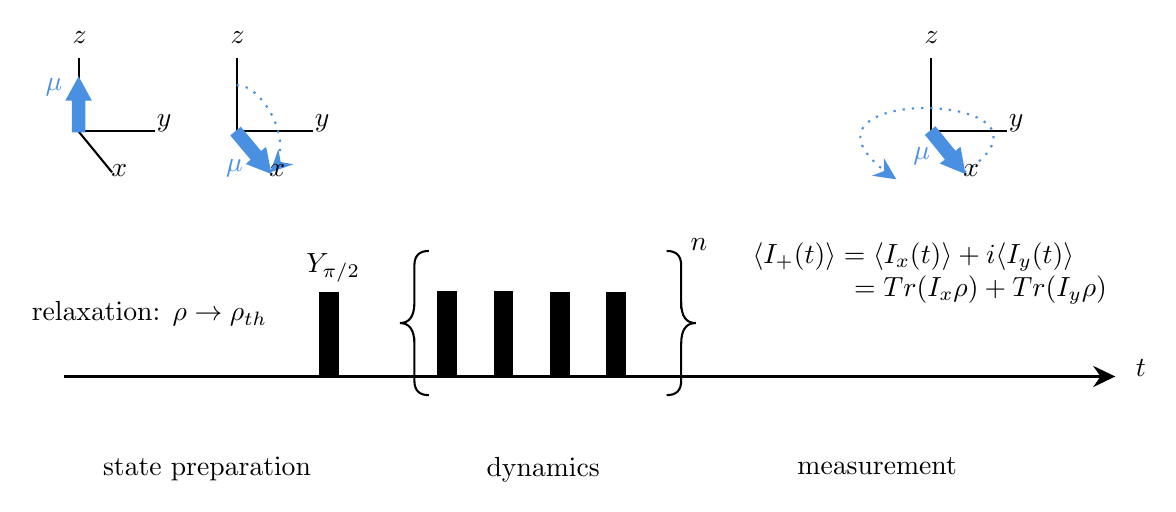
\begin{tikzpicture}[x=0.75pt,y=0.75pt,yscale=-1,xscale=1]
%uncomment if require: \path (0,339); %set diagram left start at 0, and has height of 339

%Straight Lines [id:da059464442277275764] 
\draw    (24.55,224.5) -- (528,224.5) ;
\draw [shift={(531,224.5)}, rotate = 180] [fill={rgb, 255:red, 0; green, 0; blue, 0 }  ][line width=0.08]  [draw opacity=0] (10.72,-5.15) -- (0,0) -- (10.72,5.15) -- (7.12,0) -- cycle    ;
%Shape: Rectangle [id:dp4869926759781673] 
\draw  [fill={rgb, 255:red, 0; green, 0; blue, 0 }  ,fill opacity=1 ] (147.72,184.5) -- (156.28,184.5) -- (156.28,224.5) -- (147.72,224.5) -- cycle ;
%Shape: Brace [id:dp49651760078211227] 
\draw   (200.31,164) .. controls (195.64,164) and (193.31,166.33) .. (193.31,171) -- (193.31,188.75) .. controls (193.31,195.42) and (190.98,198.75) .. (186.31,198.75) .. controls (190.98,198.75) and (193.31,202.08) .. (193.31,208.75)(193.31,205.75) -- (193.31,226.5) .. controls (193.31,231.17) and (195.64,233.5) .. (200.31,233.5) ;
%Shape: Brace [id:dp30023368862443545] 
\draw   (314.85,233.5) .. controls (319.52,233.5) and (321.85,231.17) .. (321.85,226.5) -- (321.85,208.75) .. controls (321.85,202.08) and (324.18,198.75) .. (328.85,198.75) .. controls (324.18,198.75) and (321.85,195.42) .. (321.85,188.75)(321.85,191.75) -- (321.85,171) .. controls (321.85,166.33) and (319.52,164) .. (314.85,164) ;
%Shape: Rectangle [id:dp315662766626454] 
\draw  [fill={rgb, 255:red, 0; green, 0; blue, 0 }  ,fill opacity=1 ] (204.79,184) -- (213.35,184) -- (213.35,224) -- (204.79,224) -- cycle ;
%Shape: Rectangle [id:dp17888259941747675] 
\draw  [fill={rgb, 255:red, 0; green, 0; blue, 0 }  ,fill opacity=1 ] (231.97,184) -- (240.53,184) -- (240.53,224) -- (231.97,224) -- cycle ;
%Shape: Rectangle [id:dp06356300124623626] 
\draw  [fill={rgb, 255:red, 0; green, 0; blue, 0 }  ,fill opacity=1 ] (259.14,184.5) -- (267.7,184.5) -- (267.7,224.5) -- (259.14,224.5) -- cycle ;
%Shape: Rectangle [id:dp8921611205440483] 
\draw  [fill={rgb, 255:red, 0; green, 0; blue, 0 }  ,fill opacity=1 ] (286.32,184.5) -- (294.88,184.5) -- (294.88,224.5) -- (286.32,224.5) -- cycle ;

%Straight Lines [id:da7749601125021541] 
\draw    (31.52,106.43) -- (68.16,106.43) ;
%Straight Lines [id:da8999247307947148] 
\draw    (31.52,106.43) -- (31.52,71.23) ;
%Straight Lines [id:da5729803724679712] 
\draw    (31.52,106.43) -- (47.68,126.18) ;
%Up Arrow [id:dp4684827433237555] 
\draw  [color={rgb, 255:red, 74; green, 144; blue, 226 }  ,draw opacity=1 ][fill={rgb, 255:red, 74; green, 144; blue, 226 }  ,fill opacity=1 ] (25.95,91.12) -- (31.52,80.92) -- (37.09,91.12) -- (34.31,91.12) -- (34.31,106.43) -- (28.74,106.43) -- (28.74,91.12) -- cycle ;

%Straight Lines [id:da929552293826683] 
\draw    (107.67,106.43) -- (144.3,106.43) ;
%Straight Lines [id:da7941962070301309] 
\draw    (107.67,106.43) -- (107.67,71.23) ;
%Straight Lines [id:da6780282921433607] 
\draw    (107.67,106.43) -- (123.83,126.18) ;
%Up Arrow [id:dp6006270976783238] 
\draw  [color={rgb, 255:red, 74; green, 144; blue, 226 }  ,draw opacity=1 ][fill={rgb, 255:red, 74; green, 144; blue, 226 }  ,fill opacity=1 ] (121.54,114.79) -- (123.83,126.18) -- (113.01,121.94) -- (115.14,120.15) -- (105.31,108.42) -- (109.58,104.85) -- (119.41,116.57) -- cycle ;
%Curve Lines [id:da4911151503886654] 
\draw [color={rgb, 255:red, 74; green, 144; blue, 226 }  ,draw opacity=1 ] [dash pattern={on 0.84pt off 2.51pt}]  (107.67,84.16) .. controls (119.27,83.47) and (135.41,110.02) .. (125.6,124.07) ;
\draw [shift={(123.83,126.18)}, rotate = 315] [fill={rgb, 255:red, 74; green, 144; blue, 226 }  ,fill opacity=1 ][line width=0.08]  [draw opacity=0] (10.72,-5.15) -- (0,0) -- (10.72,5.15) -- (7.12,0) -- cycle    ;

%Straight Lines [id:da7997915961213885] 
\draw    (442.02,106.43) -- (478.66,106.43) ;
%Straight Lines [id:da4153829628980219] 
\draw    (442.02,106.43) -- (442.02,71.23) ;
%Straight Lines [id:da41781258856877057] 
\draw    (442.02,106.43) -- (458.18,126.18) ;
%Up Arrow [id:dp9761066142605184] 
\draw  [color={rgb, 255:red, 74; green, 144; blue, 226 }  ,draw opacity=1 ][fill={rgb, 255:red, 74; green, 144; blue, 226 }  ,fill opacity=1 ] (456.08,114.75) -- (458.18,126.18) -- (447.44,121.76) -- (449.6,120.01) -- (439.96,108.13) -- (444.28,104.62) -- (453.92,116.5) -- cycle ;
%Curve Lines [id:da0039040723172503178] 
\draw [color={rgb, 255:red, 74; green, 144; blue, 226 }  ,draw opacity=1 ] [dash pattern={on 0.84pt off 2.51pt}]  (458.18,126.18) .. controls (519.38,85.91) and (359.75,83.05) .. (423.5,128.12) ;
\draw [shift={(425.5,129.5)}, rotate = 213.98] [fill={rgb, 255:red, 74; green, 144; blue, 226 }  ,fill opacity=1 ][line width=0.08]  [draw opacity=0] (10.72,-5.15) -- (0,0) -- (10.72,5.15) -- (7.12,0) -- cycle    ;

% Text Node
\draw (41.81,262) node [anchor=north west][inner sep=0.75pt]   [align=left] {state preparation};
% Text Node
\draw (226.6,262) node [anchor=north west][inner sep=0.75pt]   [align=left] {dynamics};
% Text Node
\draw (376.38,262) node [anchor=north west][inner sep=0.75pt]   [align=left] {measurement};
% Text Node
\draw (539.37,214.9) node [anchor=north west][inner sep=0.75pt]    {$t$};
% Text Node
\draw (154.2,172.19) node    {$Y_{\pi /2}$};
% Text Node
\draw (7.49,187) node [anchor=north west][inner sep=0.75pt]   [align=left] {relaxation: $\displaystyle \rho \rightarrow \rho _{\text{th}}$};
% Text Node
\draw (45.78,120.88) node [anchor=north west][inner sep=0.75pt]    {$x$};
% Text Node
\draw (67.69,96.81) node [anchor=north west][inner sep=0.75pt]    {$y$};
% Text Node
\draw (27.1,56.94) node [anchor=north west][inner sep=0.75pt]    {$z$};
% Text Node
\draw (14.17,79.57) node [anchor=north west][inner sep=0.75pt]  [color={rgb, 255:red, 74; green, 144; blue, 226 }  ,opacity=1 ]  {$\mu $};
% Text Node
\draw (348.12,157.4) node [anchor=north west][inner sep=0.75pt]    {$ \begin{array}{l}
\langle I_{+}( t) \rangle =\langle I_{x}( t) \rangle +i\langle I_{y}( t) \rangle \\
\ \ \ \ \ \ \ \ \ \ \ =\text{Tr}( I_{x} \rho ) +\text{Tr}( I_{y} \rho )
\end{array}$};
% Text Node
\draw (324.85,156.4) node [anchor=north west][inner sep=0.75pt]    {$n$};
% Text Node
\draw (456.28,120.88) node [anchor=north west][inner sep=0.75pt]    {$x$};
% Text Node
\draw (478.19,96.81) node [anchor=north west][inner sep=0.75pt]    {$y$};
% Text Node
\draw (437.6,56.94) node [anchor=north west][inner sep=0.75pt]    {$z$};
% Text Node
\draw (432.17,112.57) node [anchor=north west][inner sep=0.75pt]  [color={rgb, 255:red, 74; green, 144; blue, 226 }  ,opacity=1 ]  {$\mu $};
% Text Node
\draw (121.92,120.88) node [anchor=north west][inner sep=0.75pt]    {$x$};
% Text Node
\draw (143.83,96.81) node [anchor=north west][inner sep=0.75pt]    {$y$};
% Text Node
\draw (103.24,56.94) node [anchor=north west][inner sep=0.75pt]    {$z$};
% Text Node
\draw (101.09,118.36) node [anchor=north west][inner sep=0.75pt]  [color={rgb, 255:red, 74; green, 144; blue, 226 }  ,opacity=1 ]  {$\mu $};


\end{tikzpicture}
